%%%%%%%%%%%%%%%%%%%%%%%%%%%%%%%%%%%%%%%%%
% University Assignment Title Page 
% LaTeX Template
% Version 2.1 (18/10/18)
% Modified by
% Erdem TUNA &
% Halil TEMURTAŞ &
% Enes TAŞTAN
%%%%%%%%%%%%%%%%%%%%%%%%%%%%%%%%%%%%%%%%%
%
%----------------------------------------------------------------------------------------
%	PACKAGES AND OTHER DOCUMENT CONFIGURATIONS
%----------------------------------------------------------------------------------------
\documentclass[a4paper,12pt]{article}
%-----packages------
\usepackage[a4paper, total={6.2in, 9in}]{geometry}
\usepackage[english]{babel}
\usepackage[utf8x]{inputenc}
\usepackage{amsmath}
\usepackage{graphicx}
\usepackage[colorinlistoftodos]{todonotes}
\usepackage{gensymb} % this could be problem
\usepackage{float}
\usepackage{fancyref}
\usepackage{subcaption}
\usepackage[titletoc]{appendix} %appendix package
\usepackage{xcolor}
\usepackage{listings}
\usepackage{xspace}
\usepackage{amssymb}
\usepackage{nicefrac}
\usepackage{gensymb}
\usepackage{fancyhdr}
\usepackage{lipsum}  % for dummy text \lipsum[1-4]
\usepackage[final]{pdfpages}  % pdf include
%\usepackage{array} %allows more options in tables
\usepackage{pgfplots,pgf,tikz} %coding plots in latex
%\usepackage{capt-of} % allows caption outside the figure environment
\usepackage[export]{adjustbox} %more options for adjusting the images
%\usepackage{multicol,multirow,slashbox} % allows tables like table1
%\usepackage[hyperfootnotes=false]{hyperref} % clickable references
%\usepackage{epstopdf} % useful when matlab is involved
%\usepackage{placeins} % prevents the text after figure to go above figure with \FloatBarrier 
%\usepackage{listingsutf8,mcode} %import .m or any other code file mcode is for matlab highlighting
\usepackage{setspace}
%-----end of packages




%-----specifications-----
\definecolor{mGreen}{rgb}{0,0.6,0} % for python
\definecolor{mGray}{rgb}{0.5,0.5,0.5}
\definecolor{mPurple}{rgb}{0.58,0,0.82}
\definecolor{mygreen}{RGB}{28,172,0} % color values Red, Green, Blue for matlab
\definecolor{mylilas}{RGB}{170,55,241}

\setcounter{secnumdepth}{5} % how many sectioning levels to assign numbers to
\setcounter{tocdepth}{5}    % how many sectioning levels to show in ToC

\lstdefinestyle{CStyle}{
	commentstyle=\color{mGreen},
	keywordstyle=\color{magenta},
	numberstyle=\tiny\color{mGray},
	stringstyle=\color{mPurple},
	basicstyle=\footnotesize,
	breakatwhitespace=false,         
	breaklines=true,
	frame=single,
	rulecolor=\color{black!40},                 
	captionpos=b,                    
	keepspaces=true,                 
	numbers=left,                    
	numbersep=5pt,                  
	showspaces=false,                
	showstringspaces=false,
	showtabs=false,                  
	tabsize=2,
	language=C
}

\lstset{language=Matlab,%
	%basicstyle=\color{red},
	breaklines=true,%
	frame=single,
	rulecolor=\color{black!40},
	morekeywords={matlab2tikz},
	keywordstyle=\color{blue},%
	morekeywords=[2]{1}, keywordstyle=[2]{\color{black}},
	identifierstyle=\color{black},%
	stringstyle=\color{mylilas},
	commentstyle=\color{mygreen},%
	showstringspaces=false,%without this there will be a symbol in the places where there is a space
	numbers=left,%
	numberstyle={\tiny \color{black}},% size of the numbers
	numbersep=9pt, % this defines how far the numbers are from the text
	emph=[1]{for,end,break},emphstyle=[1]\color{red}, %some words to emphasise
	%emph=[2]{word1,word2}, emphstyle=[2]{style},    
}


\tikzset{
	desicion/.style={
		diamond,
		draw,
		text width=4em,
		text badly centered,
		inner sep=0pt
	},
	block/.style={
		rectangle,
		draw,
		text width=10em,
		text centered,
		rounded corners
	},
	cloud/.style={
		draw,
		ellipse,
		minimum height=2em
	},
	descr/.style={
		fill=white,
		inner sep=2.5pt
	},
	connector/.style={
		-latex,
		font=\scriptsize
	},
	rectangle connector/.style={
		connector,
		to path={(\tikztostart) -- ++(#1,0pt) \tikztonodes |- (\tikztotarget) },
		pos=0.5
	},
	rectangle connector/.default=-2cm,
	straight connector/.style={
		connector,
		to path=--(\tikztotarget) \tikztonodes
	}
}

\tikzset{
	desicion/.style={
		diamond,
		draw,
		text width=4em,
		text badly centered,
		inner sep=0pt
	},
	block/.style={
		rectangle,
		draw,
		text width=10em,
		text centered,
		rounded corners
	},
	cloud/.style={
		draw,
		ellipse,
		minimum height=2em
	},
	descr/.style={
		fill=white,
		inner sep=2.5pt
	},
	connector/.style={
		-latex,
		font=\scriptsize
	},
	rectangle connector/.style={
		connector,
		to path={(\tikztostart) -- ++(#1,0pt) \tikztonodes |- (\tikztotarget) },
		pos=0.5
	},
	rectangle connector/.default=-2cm,
	straight connector/.style={
		connector,
		to path=--(\tikztotarget) \tikztonodes
	}
}
%-----end of specifications-----


%----commands----
\newcommand\nd{\textsuperscript{nd}\xspace}
\newcommand\rd{\textsuperscript{rd}\xspace}
\newcommand\nth{\textsuperscript{th}\xspace} %\th is taken already
\newcommand{\specialcell}[2][c]{ \begin{tabular}[#1]{@{}c@{}}#2\end{tabular}} % for too long table lines

\newcommand{\blankpage}{
	\- \\[9cm]	
	{ \centering \textit{This page intentionally left blank.} \par }
	\- \\[9cm]
}% For Blank Page

\makeatletter
\renewcommand\paragraph{\@startsection{paragraph}{4}{\z@}%
	{-2.5ex\@plus -1ex \@minus -.25ex}%
	{1.25ex \@plus .25ex}%
	{\normalfont\normalsize\bfseries}}
\makeatother
%-----end of commands-----
\onehalfspacing
\begin{document}

\begin{titlepage}

\newcommand{\HRule}{\rule{\linewidth}{0.5mm}} % Defines a new command for the horizontal lines, change thickness here
\centering 


\includegraphics[width=\textwidth,height=\textheight,keepaspectratio]{../../../Documents/logos/logo3-with-stroke}\\[0.5cm]

\textsc{\LARGE Middle East Technical University}\\[0.5cm] % Name of your university/college
\textsc{\Large Department of \\Electrical and Electronics Engineering }\\[0.5cm] % Major heading such as course name
\textsc{\large EE493 ENGINEERING DESIGN I}\\[0.5cm] % Minor heading such as course title


\HRule \\[0cm]
{ \huge \bfseries  Car Chasing Robot\\[0.1cm] \LARGE \bfseries Conceptual Design Report}\\[0cm] % Title of your document
\HRule \\[1cm]

\begin{minipage}[l]{0.6\textwidth}
\raggedright
		\large{\textbf{Supervisor:}}	Assoc. Prof. Emre Özkan \\
		\hspace{3.05cm}  METU EE / C-112

\end{minipage}
\begin{minipage}[r]{0.35\textwidth}
\raggedright
		\textbf{Project Start:} 4/10/2018\\
		\textbf{Project End:} \ \  26/5/2019\\
		\textbf{Project Budget:} \$450

\end{minipage}\\[1cm]
\begin{minipage}{\textwidth}
	\begin{flushleft}
		\large{\textbf{Company Name :}}	Duayenler Ltd. Şti.\\
		\begin{table}[H]
			\begin{tabular}{l l l l}
				\hline
				\textbf{Members}&\textbf{Title}& \textbf{ID}&\textbf{Phone} \\ \hline
				Sarper Sertel & Electronics Engineer& 2094449 & 0542 515 6039  \\ 
				Enes Taştan & Hardware Design Engineer & 2068989 & 0543 683 4336  \\ 
				Erdem Tuna & Embedded Systems Engineer& 2617419 & 0535 256 3320  \\ 
				Halil Temurtaş & Control Engineer& 2094522 & 0531 632 2194  \\
				İlker Sağlık & Software Engineer& 2094423 & 0541 722 9573  \\ \hline
				
				
			\end{tabular}
		\end{table}
	\end{flushleft}
\end{minipage}\\[1cm]

\begin{flushbottom}
{\large December 26, 2018} % Date, change the \today to a set date if you want to be precise
\end{flushbottom}

\end{titlepage}

\blankpage
\tableofcontents
\newpage

\section{Executive Summary}

	Increasing demand on automobiles, encourages industry to produce more. The increase of car count in the traffic, makes the traffic flow more complex. In this scope, autonomous cars bring an innovative solution for reducing the complexity. Potential benefits of automated cars include smart use of fuel, safer traffic and increased mobility. To realize and come up with such solutions, DUAYENLER Ltd. Şti. (DUAYENLER) is founded by five innovative and enthusiast electronics engineering students to intelligently automate the future of traffic.\\
	
	DUAYENLER is composed of talented and diligent people from different disciplines to complete the envisioned problem. DUAYENLER consists of two engineers from computer area, two from electronics area and one from control area. Since realization of the problem requires combinations of different disciplines, DUAYENLER is qualified to accomplish the encountered problems.\\
	
	DUAYENLER will address the need of autonomous cars. Thus, the aim of the proposed project is to design and construct a vehicle that can follow a closed path without a driver on board. Furthermore, the vehicle will be able to sense other vehicles on the road as well as handling the obstacles.\\
	
	The vehicle will use camera vision and sensors to detect and understand environment. With the obtained data, the vehicle will operate in a way that it adjusts its direction and speed correctly. Additionally, if the vehicle detects another vehicle within 5 cm either at the front or at the back, it will activate the handshake protocol to communicate with the opponent and stop with positive signal.\\
	
	The duration of the project is intended to last 33 weeks, starting from October, 1 2019 and ending in May, 26 2019. The estimated cost for research and development phase is  \$ 450 whereas mass production cost per vehicle will be at most \$ 200. Along with the vehicle itself, DUAYENLER will provide its customers with deliverables such as user and technical manuals, elliptical race path, chargeable battery and battery charger. Also, the vehicle will have two (2) years of warranty.
	

\section{Introduction}

	Driving is a common event that many people experience in their daily life. As time passes, human reflexes started to become insufficient for driving compared to fast pace of daily life in modern world. Together with the developments in the technology, new solutions are proposed to assist the driver such as lane tracking and emergency breaking systems. The ultimate version of such solutions are considered to be fully autonomous self-driving cars. \\

Self-driving vehicles are presented to the society as a solution that can facilitate people's life in many ways. Fast operation of the electronics system allows faster response than humans can. A fast and a reliable operation of self-driving action can prevent many accidents and increase the safety of the roads in heavy traffics since the system is immune to human defects such as distraction and panic. As a result, autonomous vehicles can open doors to a safer and more conventional future.\\

DUAYENLER Ltd. Şti.(DUAYENLER) is launched with the aim of innovating automation technologies. In that context, a device that can detect the road and other vehicles on them will be built. It autonomously track the lane and stay on the road while trying to be as fast as possible.\\

This report includes;
\begin{itemize}
	\item Organization of the company by explaining of the qualifications of the members. \vspace{-.2cm}
	\item Requirements for physically realizing the intended vehicle \vspace{-.2cm}
	\item Possible solutions in system and subsystem levels by explaining their operations\vspace{-.2cm}
	\item Timeline and estimated budget of the project\vspace{-.2cm}
	\item Expected deliverables of the project \vspace{-.2cm}
\end{itemize} 



\section{The Team}

	DUAYENLER was founded in September 2018 by five electrical and electronics engineering students from Middle East Technical University. The company structure is shown in \textit{Figure~\ref{fig:company_tree}}. The team is composed of variously skilled visionary members. The leader of the team is Halil Temurtaş, a control engineer.\\
	
	Being the team leader, Halil manages the organization of the members as well as drawing an outline for the future calendar. He is experienced in using microcontrollers, device testing and project scheduling. He has experience in TAI as an intern engineer in product testing and in product design in "Very Light Aircraft" project that gives him the understanding of the project management. And his EE300 summer practice, he gained experience in using Raspberry Pi and Arduino while building a sun follower robot. He will be working on the development of the subsystems computation, motion and driving in parallel with his experiences.\\
	
	Sarper Sertel, electronics engineer, has a wide understanding of microelectronics circuits and their design as well as analog lumped circuits. He has experience in electronic maintenance of jet fighters which includes sensors and electromechanical systems integration. He has also experience in  analog circuit design, specifically power electronics, which can be useful in designing driving unit elements. He is also interested in mechanical systems such as structure organization.\\
	
	Enes Taştan, hardware design engineer, has experience in many types of mechanical works such as assembly and repair works from family business. In addition, he worked on PCB design of power electronics circuits in his internship. He is interested in control of electromechanical systems. Considering his specializations, driving, motion and structure unit can be listed as most relevant subsystem he can work on.\\
	
	Erdem Tuna, embedded systems engineer, is experienced in use of microcontrollers with sensors and wireless communication between them. He also simulated 4G and 5G mobile networks using C++ based open source software. Thus, he is experienced in programming and will be contributing to subsystems requiring coding and developing algorithms. He will take part in computation and sensing subsystems.\\
	\\
	
	İlker Sağlık, software engineer, is also interested in programming and microcontrollers. He has some programming experiences with different languages such as C,C++,Verilog, Assembly etc. He also has experiences with coding with Arduino using sensors. In his internship, he worked for the communication protocols between radars. He will be working on sensing and driving subsystems.

\begin{figure}[t!]
	\centering
	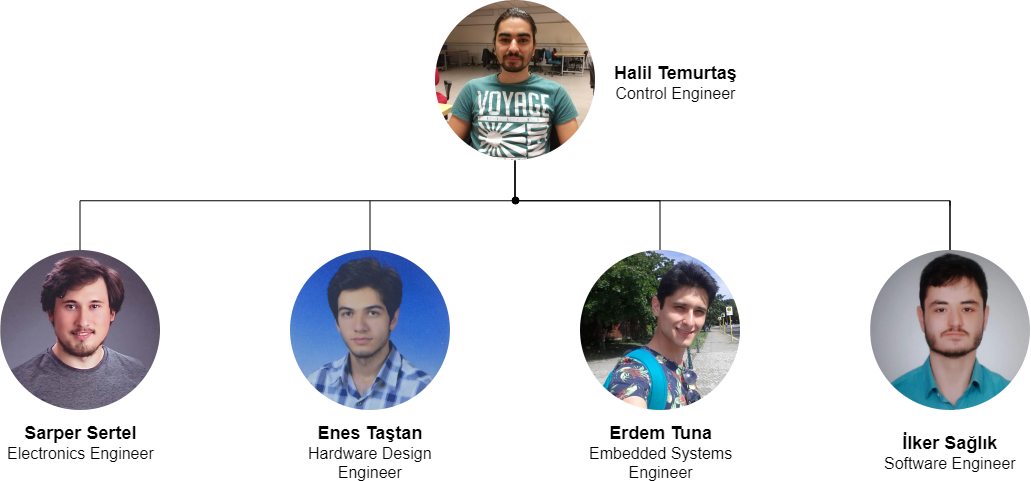
\includegraphics[width=\textwidth,height=\textheight,keepaspectratio]{../../../Documents/company/company-tree} 
	\caption{\label{fig:company_tree}Company Tree of DUAYENLER.}
\end{figure}


\newpage

		
	\begin{table}[H]
		\centering
		\caption{\label{tab:project_eval}Project Evaluation Chart}\vspace{-.2cm}
%		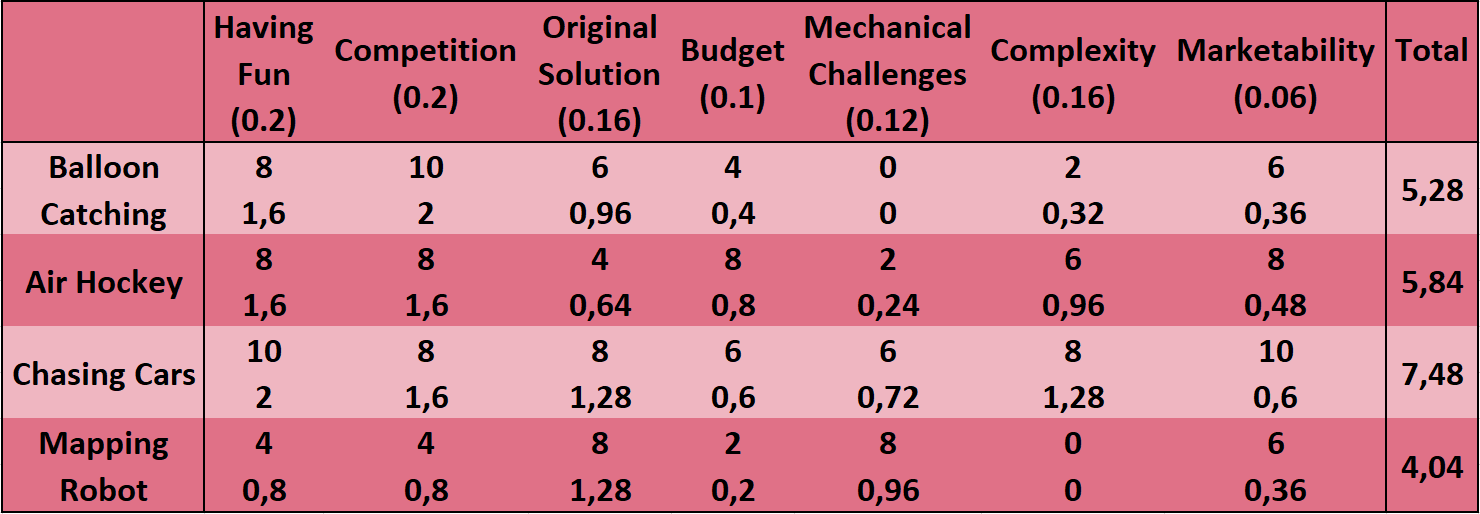
\includegraphics[width=\textwidth,height=\textheight,keepaspectratio]{images/project_evaluation4} 
	\vspace*{-.9cm}	\begin{center}
		{\small 0: Failure, 2: Unacceptable, 4: Average, 6: Satisfactory, 8: Good, 10: Excellent }	
		\end{center}
	\end{table}	\vspace*{-.5cm}	
	
	
	
	
	\begin{table}[H]
		\centering
		\caption{\label{tab:sub_project_objective_tree}Pairwise Comparison Charts for Sub-Objectives}\vspace{-.2cm}
%		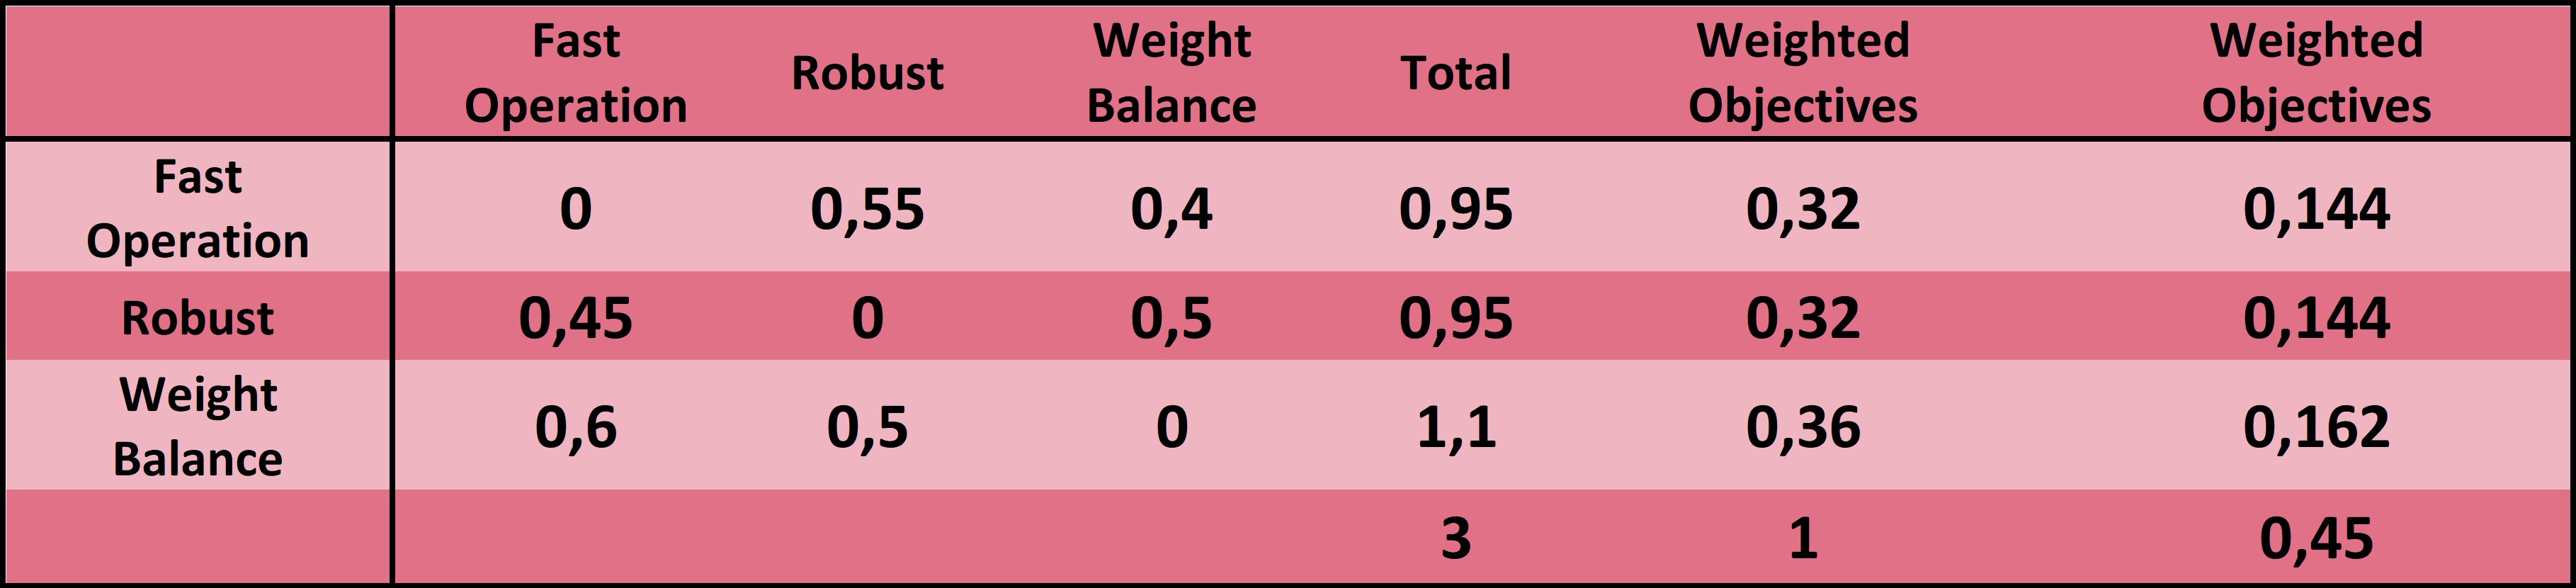
\includegraphics[width=\textwidth,height=\textheight,keepaspectratio]{images/proje_objective_tree_2a} 
	\vspace*{-.9cm}	\begin{center}
		{\small 0-0.2: No Importance, 0.2-0.4: Less Importance, 0.4-0.6: Equal Importance,\\ 0.6-0.8: More Importance, 0.8-1: Absolute Importance }	
		\end{center}
	\end{table}	\vspace*{-.5cm}
	
	
	
	
	\subsection{Systems \& Subsystems of Chosen Project}
	
\newpage

\section{Conclusion}
As technology develops further, the automated robotics can ease the human life by finding solutions to daily problems. Driving is one of these problems. Many companies are trying to solve this problem by pushing the limits of the robotics area. DUAYENLER, as a visionary company in this field, will produce a fast-autonomous car that is trying to catch the opponent in its elevated elliptical path.\\

As in every project, creating an autonomous car has some problems that must be considered; such as staying on the path, implementation of the handshake protocol with the opponent robot, being fast and robust. However, there are some solution alternatives. For example, to keep the robot in the path, image processing or sensor arrays can be used. For the faster and robust movement of the car, more capable DC motors such as brushed DC motors and a 4-wheeled car structure with servos on the front can be used. To carry out the handshake protocol with the opponent, Bluetooth modules working in accordance with a distance sensor can be used.\\

According to DUAYENLER, the major objectives are fast operation, robustness, weight balance and low power consumption. Since the main aim is catching the opponent without losing the path, the fast operation and robustness are very important. Also, low power consumption is another objective that should be common for all the companies.\\

DUAYENLER believes that the result will bring an innovative approach to the design of autonomous cars because it not only has the self-driving capability, but also the capability of communicating with the opponent.

\newpage
\begin{appendices}
	
%%		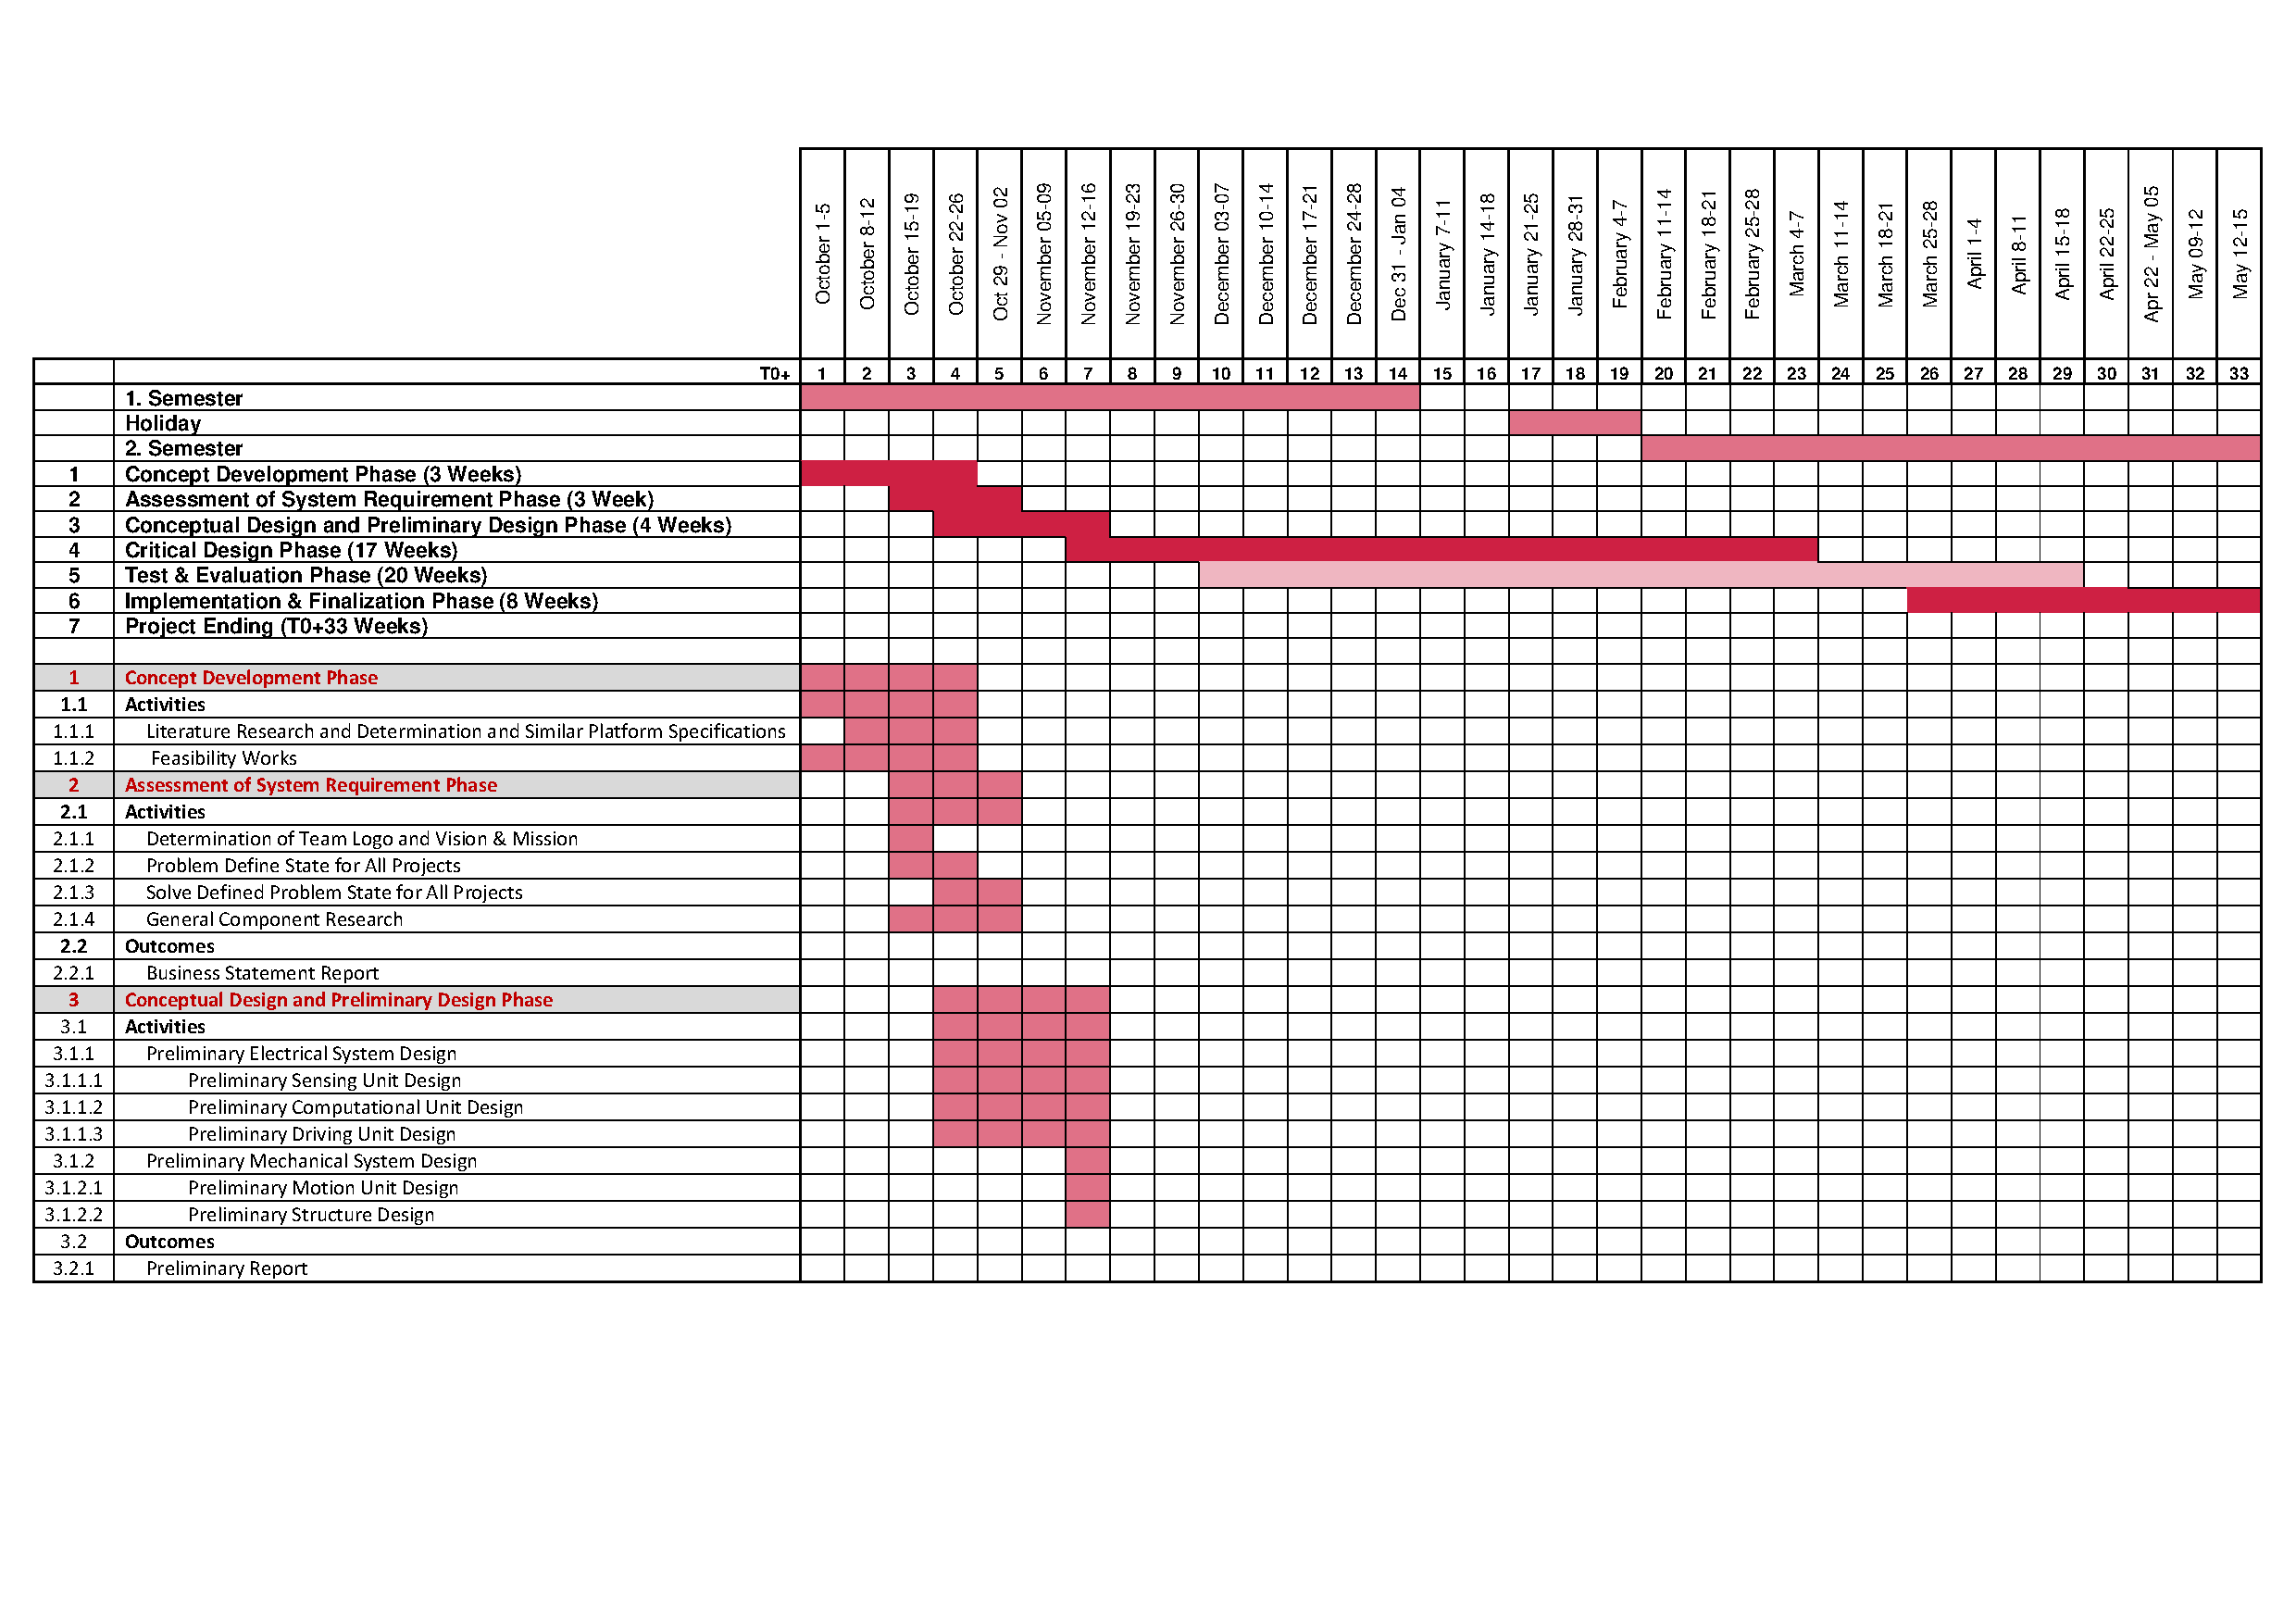
\includepdf[landscape=true,pages=1, scale=0.775,angle=0,pagecommand=\section{Gannt Chart}]{gannt2.pdf}
%%		\includepdf[landscape=true,pages=2, scale=0.775,angle=0,pagecommand=]{gannt2.pdf}

	
\end{appendices}




\end{document}

%----samples------
%\begin{itemize}
%\item Item
%\item Item
%\end{itemize}

%\begin{figure}[H]
%\center
%\setlength{\unitlength}{\textwidth} 
%
\includegraphics[width=0.7\unitlength]{images/logo1}
%\caption{\label{fig:logo}Logo }
%\end{figure}

%\begin{figure}[H]
%	\setlength{\unitlength}{\textwidth} 
%	\centering
%	\begin{subfigure}{.5\textwidth}
%  		\centering
%  		
\includegraphics[width=0.48\unitlength]{images/logo1}
%  		\caption{\label{fig:logo1}Logo1 }
%	\end{subfigure}%
%	\begin{subfigure}{.5\textwidth}
%  		\centering
%		
\includegraphics[width=0.48\unitlength]{images/logo2}
%  		\caption{\label{fig:logo2}Logo2}
%	\end{subfigure}
%\caption{\label{fig:calisandegree} Small Logos   }
%\end{figure}
	
%\begin{table}[H]
%  \centering
% 
%    \begin{tabular}{c|c|c}
%       $$A$$ & $$B$$ & $$C$$ \\ \hline
%       1 & 2 & 3  \\ \hline
%       2 & 3 & 4  \\ \hline
%       3 & 4 & 5  \\ \hline
%       4 & 5 & 6  
%      
%  \end{tabular}
%  \caption{table}
%  \label{tab:table}
%\end{table}
	
%\begin{table}[H]
%  \centering
% 
%    \begin{tabular}{c|c|c}
%       \backslashbox{$A$}{$a$} & $$\specialcell{ Average deviation \\ after subtracting out the  \\ frequency error }$$ & $$C$$ \\ \hline
%       \multirow{2}{*}{1} & 2 & 3  \\ \cline{2-3}
%        & 3 & 4  \\ \hline
%       3 & \multicolumn{2}{c}{4}  \\ \hline
%       4 & 5 & 6  
%      
%  \end{tabular}
%  \caption{table}
%  \label{tab:table}
%\end{table}
%-----end of samples-----